\documentclass[letterpaper,headings=standardclasses]{scrartcl}

\usepackage[margin=1in,includefoot]{geometry}
\usepackage{amssymb}
\usepackage{amsmath}
\usepackage{listings}
\usepackage{tikz}
\usepackage{float}

\usetikzlibrary{shapes,arrows}

\tikzset{
  block/.style    = {draw, thick, rectangle, minimum height = 3em, minimum width = 3em},
  sum/.style      = {draw, circle},
  input/.style    = {coordinate, circle},
  output/.style   = {coordinate, circle}
}

\lstset{basicstyle=\ttfamily,language=python,columns=flexible,breaklines=true,showstringspaces=false}

\DeclareMathOperator{\sgn}{sgn}

\title{Homework 8}
\subtitle{CS 559 - Neural Networks - Fall 2019}
\author{Matteo Corain 650088272}

\begin{document}

\maketitle

\section{Question 1}

\subsection{Centroids generation}

The centroids generation step is carried out using the provided implementation of the $k$-means algorithm, where $k = 10$ both for the positive class and the negative class (20 centers in total were generated). The \texttt{kmeans()} procedure has been coded for this purpose, receiving as arguments the value of $k$ and the list of training samples $x_i$, $i = 1, \dots, 100$, randomly generated in $\left[ 0,1 \right]^2$. This performs the following steps:

\begin{itemize}
    \item It initializes the set of centroids by drawing $k$ random points from the input space, storing them in the \texttt{centers} list;
    \item It computes the nearest centroid for each sample, storing the associations in the \texttt{classes} list;
    \item It starts a loop until the \texttt{unchanged} flag goes to zero; for each iteration:
    \begin{itemize}
        \item It recomputes each centroid by averaging all the points in the associated Voronoi region, defined by the points that were assigned to that centroid in the previous iteration; if no points are associated to the considered centroid (operation that returns a division by zero error), a new centroid is randomly initialized;
        \item It computes the new nearest centroid for each sample, storing the associations in the \texttt{new\_classes} list;
        \item It checks whether the \texttt{classes} and \texttt{new\_classes} lists are the same and set the result of the comparison to the value of \texttt{unchanged};
        \item It copies back the new classes on the \texttt{classes} list.
    \end{itemize}
    \item At the end of the loop, the procedure returns the list of centers and the index of the closest center for each sample.
\end{itemize}

The \texttt{kmeans()} procedure is applied separately to the list of points in the positive and negative classes; finally, an overall list of centroids is produced by concatenation of the returned results. The obtained clustering is shown in figure \ref{data_20}.

\begin{figure}[h]
    \centering
    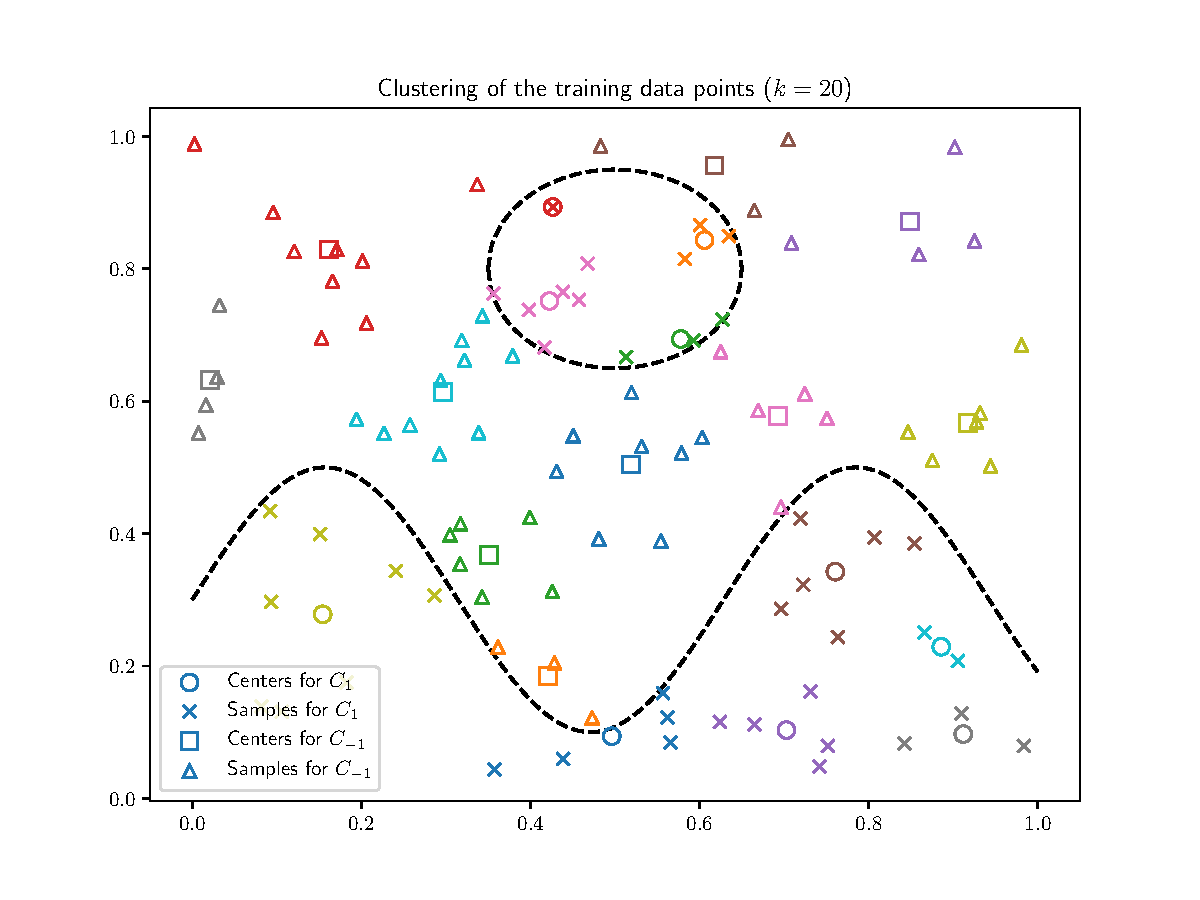
\includegraphics[width=0.7\linewidth]{data_20.pdf}
    \caption{Clustering of the training data points ($k = 20$)}
    \label{data_20}
\end{figure}

\subsection{Radial basis function mapping}

The centroids computed at the previous steps have been used to map the original data points into an appropriate higher dimensional space, by means of an opportune radial basis function $\phi(x, \mu)$. For the sake of the exercise, a Gaussian RBF has been used:

$$ \phi(x, \mu) = e^{-\beta ||x - \mu||^2} $$

Where $\beta$ is a free parameter (sometimes defined in terms of the standard deviation of the data), $x$ is one of the considered samples and $\mu$ is one of the computed centroids. In this case, each of the 2-dimensional samples was mapped on a 20-dimensional vector defined as:

$$ x' = \left[ \begin{matrix} \phi(x, \mu_1) \\ \vdots \\ \phi(x, \mu_{20}) \end{matrix} \right] = \left[ \begin{matrix} e^{-\beta ||x - \mu_1||^2} \\ \vdots \\ e^{-\beta ||x - \mu_{20}||^2} \end{matrix} \right] $$

As for the parameter $\beta$, two possible values were tested ($\beta_1 = 1, \beta_2 = 10$) in order to analyze its effect on the overall results. In code, the mapping procedure is implemented in the \texttt{rbfmap()} function, which takes as arguments the sample to map, the list of centroids and the value of $\beta$.

\subsection{Perceptron training}

The RBF-mapped representations of the original samples have been used for the supervised training a perceptron with 20 inputs (21, if we consider also the bias-related input $x_0 = 1$), in the hope that they were linearly separable in the RBF space. For the training step, a mostly standard perceptron training algorithm has been used, with a few notable differences:

\begin{itemize}
    \item Since in the original version of the PTA the considered perceptron use step activation (while here it uses signum activation), the shorthand formula for weight update was split into two separate update rules:
    \begin{itemize}
        \item The first is applied when $d_i = 1$ but $y_i = \sgn{(wx_i)} = -1$:
        $$ w \gets w + \eta x_i $$ 
        \item The other is applied when $d_i = -1$ but $y_i = \sgn{(wx_i)} = 1$:
        $$ w \gets w - \eta x_i $$
    \end{itemize}
    In this way, we avoid the introduction of an additional factor of 2 which may cause convergence problems by effectively doubling the value of the configured learning rate.

    \item An update rule for $\eta$, which reduces the value of the learning rate of a 0.9 factor when the errors increase from an epoch to the other, has also been introduced for avoiding oscillations and allowing for faster convergence.
\end{itemize}

The perceptron training algorithm has been coded in the \texttt{pta()} function, receiving as arguments the value of the initial learning rate, the initial weights vector, the training set (whose elements have the first component set to 1 to account for the bias-related input), the expected outputs and the epoch limit value after which the algorithm terminates even if convergence has not been reached; the procedure returns the trained weights vector, the number of training epochs and the number of misclassifications per epoch.

\subsection{Results}

A first attempt was initially performed by setting parameters $\beta$ to 1, $\eta$ to 0.1, epoch limit to 5000 and by drawing the initial weights for the PTA from a uniform distribution in $[-1, 1]$. In this case, however, the algorithm was not able to converge within the configured epoch limit, remaining fairly stable at around 30 misclassifications after the first epochs. Consequently, the obtained boundary (shown in figure \ref{sep_20_1}) was very different from the expected one, presenting a large number of misclassified items from both classes.

\begin{figure}[h]
    \centering
    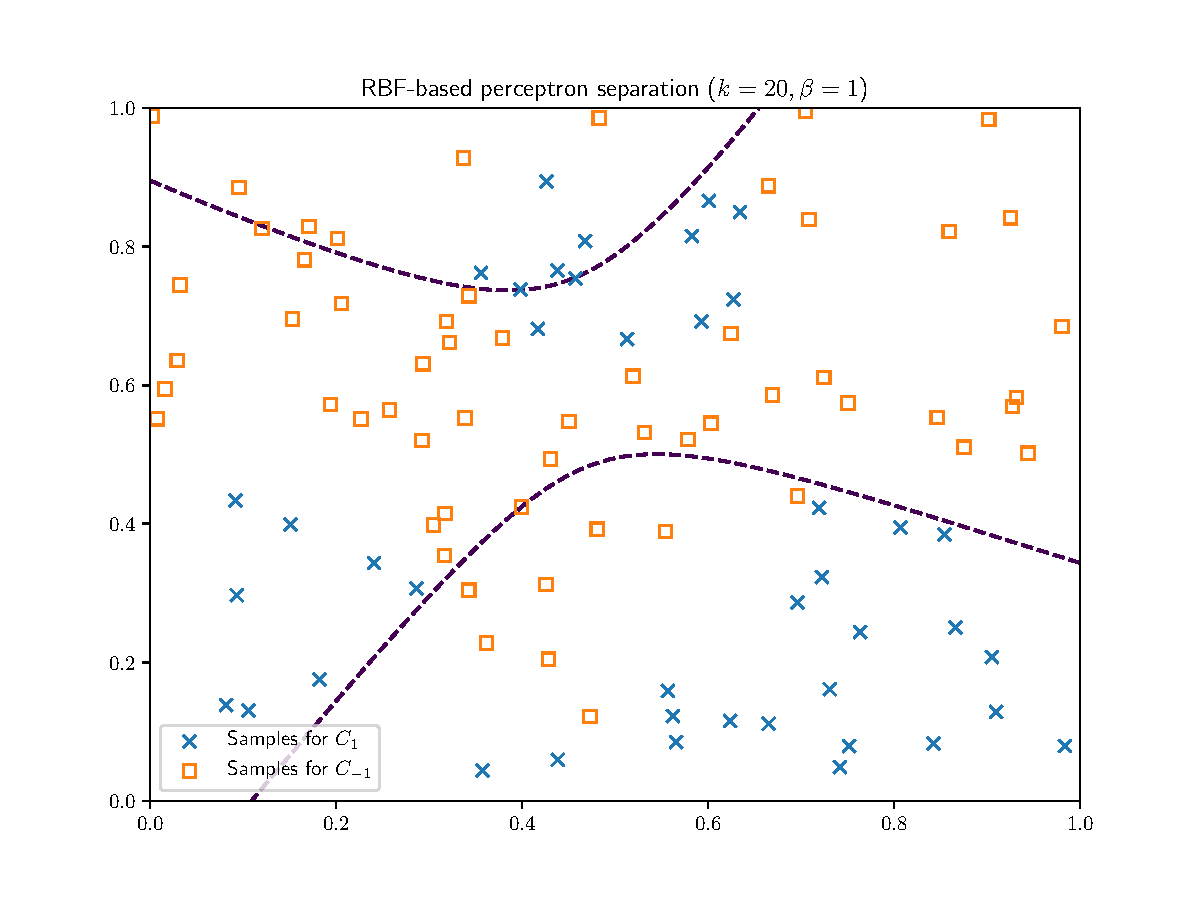
\includegraphics[width=0.7\linewidth]{sep_20_1.pdf}
    \caption{RBF-based perceptron separation ($k = 20$, $\beta = 1$)}
    \label{sep_20_1}
\end{figure}

The conclusion we can draw from this is that our RBF mapping is not good enough to make our patterns separable in the RBF space. In particular, we can notice that, since our training samples are drawn from $[0,1]^2$, the maximum distance between a point and a centroid can be no more than $\sqrt{2}$ (when they are in two opposite vertices of the considered region), and in practice it is generally much less than that (it is very unlikely for such a distribution of data to happen). When we map our data points into the RBF space, each feature $x_i'$ of the mapped point will consequently satisfy the following inequality:

$$ e^{-\max{||x - \mu||^2}} = e^{-2} = 0.1353 \le x_i' \le 1 = e^{0} = e^{-\min{||x - \mu||^2}} $$

In other words, the mapped data points be confined in the $[e^{-2}, 1]^{20}$ sub-region of the ``complete'' mapping space $(0,1]^{20}$ (0 is excluded since we assume that $\max{||x - \mu||^2} < \infty$), effectively losing a very large portion of the RBF space. For this reason, we have to reconsider the way our patterns are mapped to the RBF space; an obvious choice of intervention is on parameter $\beta$, which in the second run was significantly increased to the value of 10. In this way, almost the entire mapping space can be used (since $e^{-20} = 2 * 10^{-9}$, leading to a very limited loss in terms of excluded volume); thus, we can expect that our patterns will be more likely to be linearly separable.

Running the script using $\beta = 10$ and leaving all the other parameters to their previous values, PTA was able to converge in a relatively small number of epochs (90), sign that, by exploiting almost the entirety of our mapping space, our patterns become clearly separable by a linear classifier. Results for this second run are shown in figure \ref{sep_20_10}.

\begin{figure}[h]
    \centering
    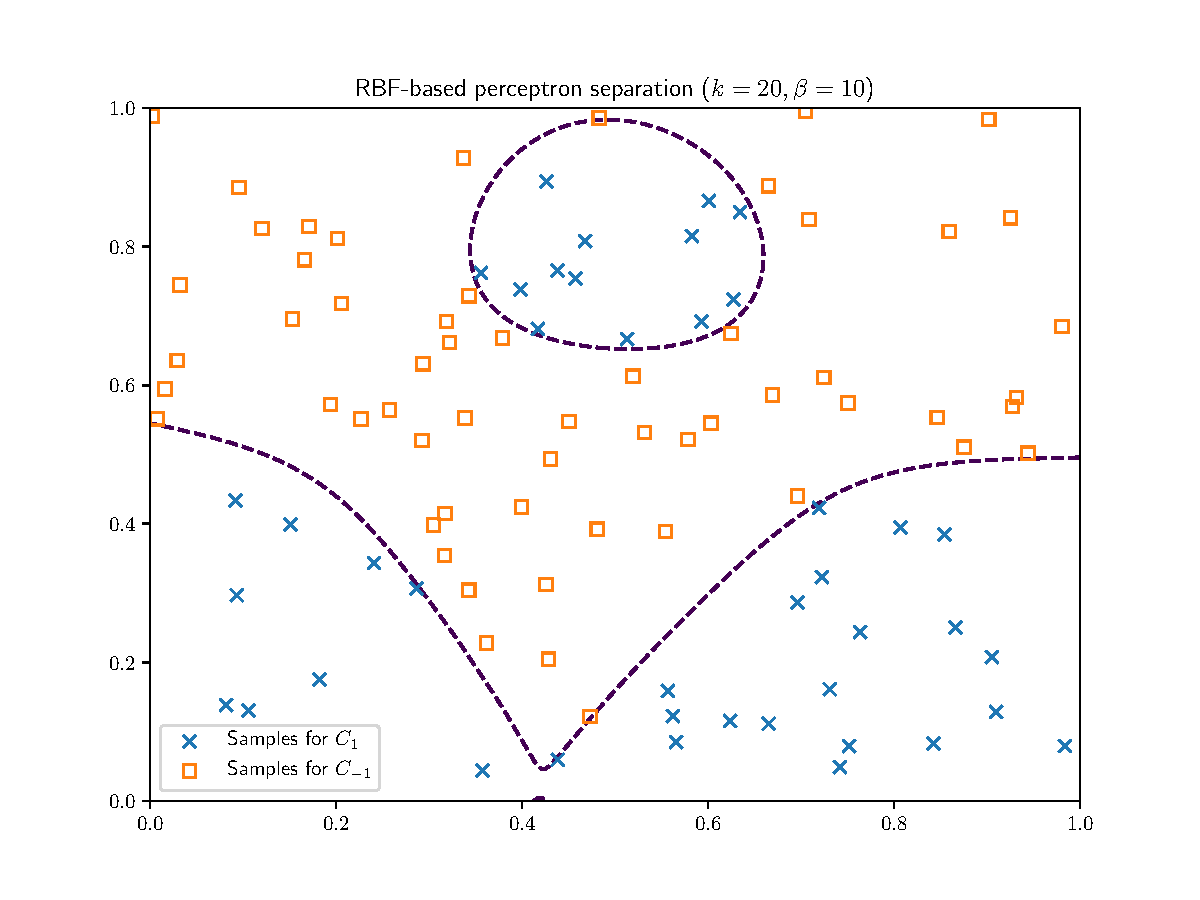
\includegraphics[width=0.7\linewidth]{sep_20_10.pdf}
    \caption{RBF-based perceptron separation ($k = 20$, $\beta = 10$)}
    \label{sep_20_10}
\end{figure}

\subsection{Differences with the case $k = 4$}

A third run was finally performed, using the same value of $\beta = 10$ as before but setting the value of $k$ to 2 for both runs of the $k$-means algorithm (for the positive and the negative classes). Again, the PTA was not able to reach convergence within the configured epoch limit, showing large oscillations in the number of misclassifications throughout the different epochs.

From this, we can conclude that, in this case as well, our mapping is not good enough to make the classes linearly separable; this is also reflected by the obtained separator, which appears to be significantly different from the original one and not able to divide the data points clearly. Results of the $k$-means clustering procedure and the separation obtained by running PTA are shown in figures \ref{data_4} and \ref{sep_4_10}.

\begin{figure}[h]
    \centering
    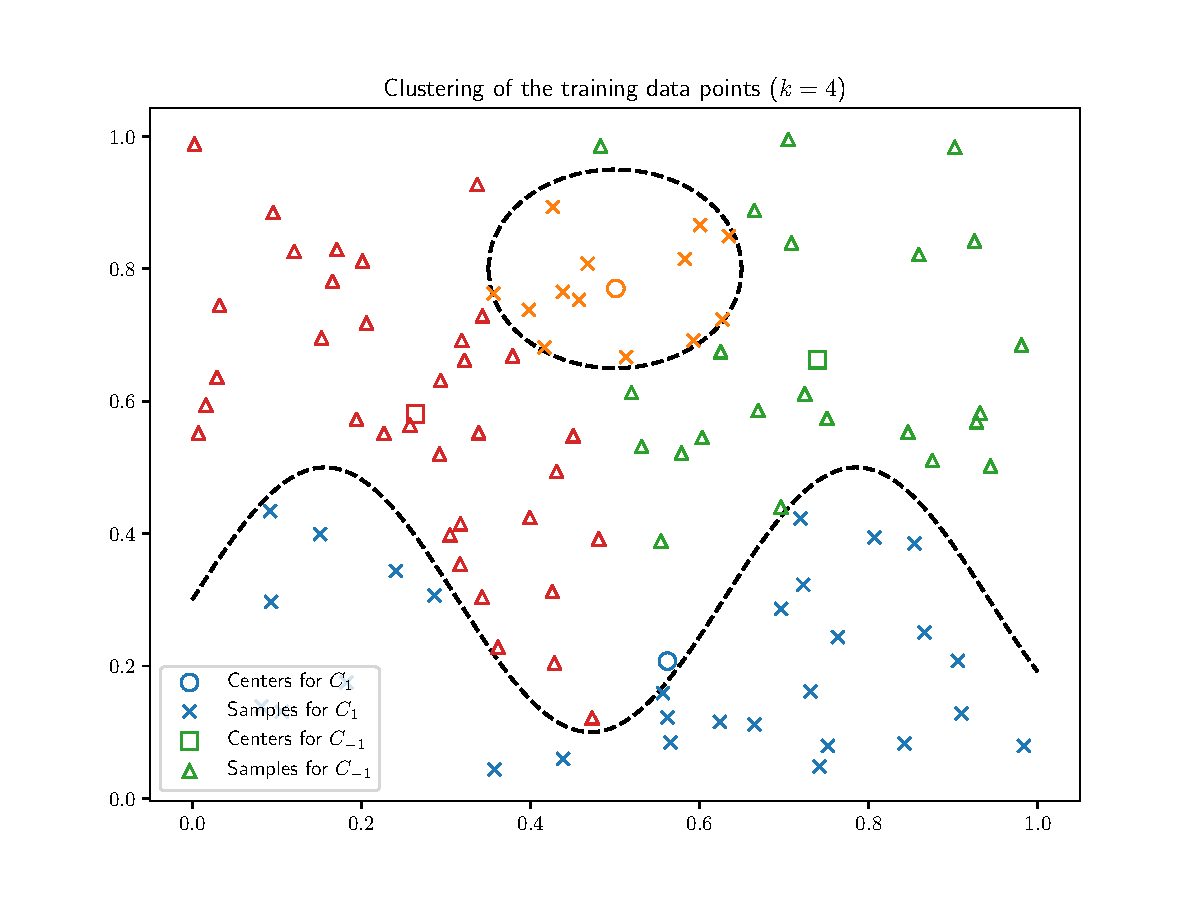
\includegraphics[width=0.7\linewidth]{data_4.pdf}
    \caption{Clustering of the training data points ($k = 4$)}
    \label{data_4}
\end{figure}

\begin{figure}[h]
    \centering
    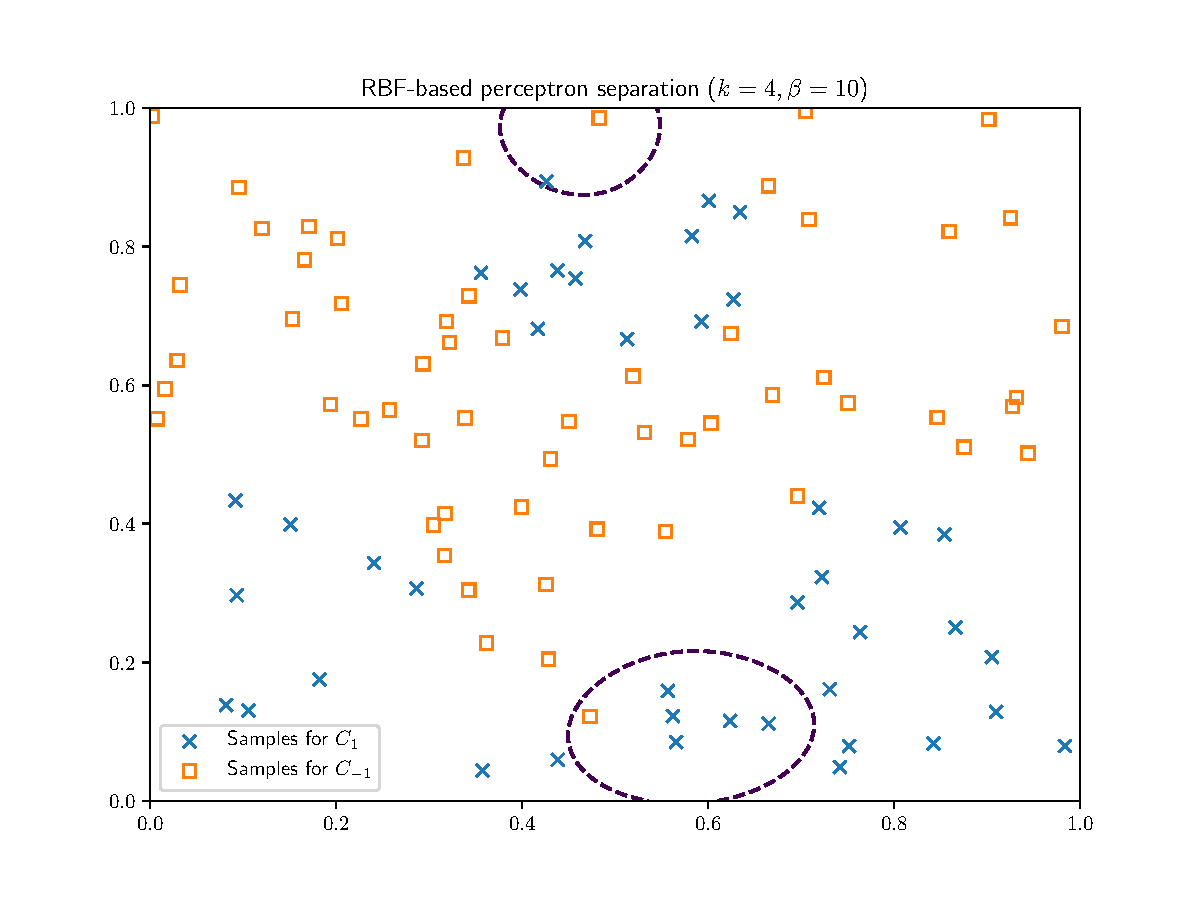
\includegraphics[width=0.7\linewidth]{sep_4_10.pdf}
    \caption{RBF-based perceptron separation ($k = 4$, $\beta = 10$)}
    \label{sep_4_10}
\end{figure}

\subsection{Complete Python code}

\lstinputlisting[basicstyle=\ttfamily\scriptsize]{hw8.py}

\end{document}